\paragraph{nonnative-sub}

\subparagraph{target}
Check the substract relation among three nonnative target objects.

\subparagraph{Constraints logic}
\begin{itemize}
    \item Check equation for gadget: \verb|diff + b = a + modular * overflow|;
    \item Check that ``overflow is bool'';
    \item Check that ``diff.limbs is range U32''.
\end{itemize}

\subparagraph{Process layout}
See \figref{fig:nonnative-sub-layout}
\begin{figure}[!ht]
    \centering
    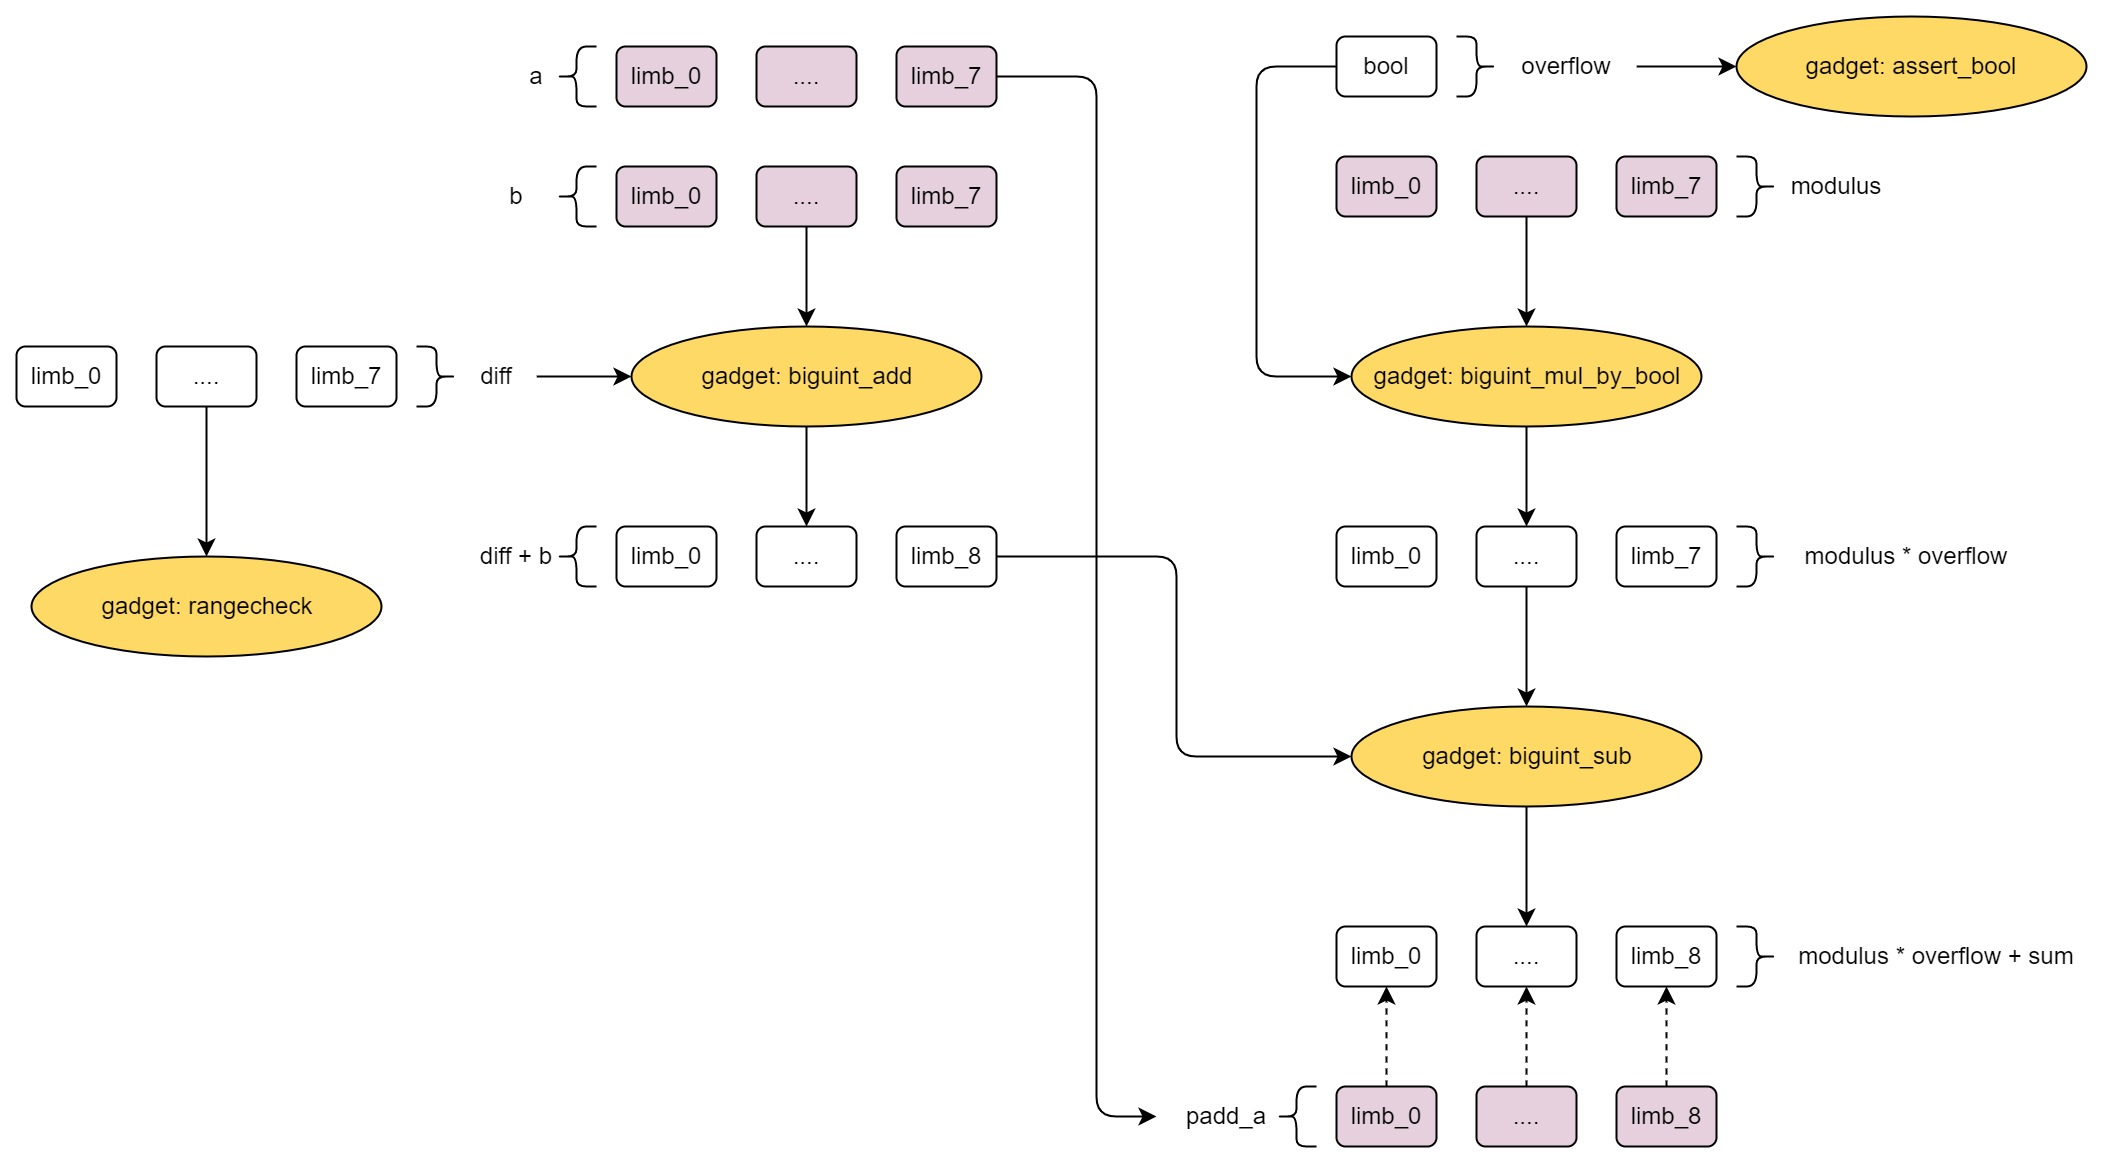
\includegraphics[width=0.8\textwidth]{nonnative-sub-layout.jpg}
    \caption{nonnative-sub layout}
    \label{fig:nonnative-sub-layout}
\end{figure}

\subparagraph{Constraints info and costs}
\begin{itemize}
    \item gadget biguint-add num: 1
    \item gadget biguint-sub num: 1
    \item gadget biguint-mul-by-bool num: 1
    \item gadget u32rangecheck num: 1
    \item gadget assert-bool num: 1
    \item gate type num: 4(U32AddManyGate, U32SubtractionGate, U32RangeCheckGate, ArithmeticGate)
    \item gate instance num: 7 = 2(U32AddManyGate) + 2(U32SubtractionGate) + 1(U32RangeCheckGate) + 1(ArithmeticGate(1,0)) + 1(ArithmeticGate(1,-1))
    \item copy-constraints: 89 = 32{biguint-add num} + 27{U32SubtractionGate} + 9{biguint-mul-by-bool} + 8{u32rangecheck} + 4{assert-bool} + 9
\end{itemize}

\subparagraph{Questions}
\begin{itemize}
    \item Why not constraint for overflow at nonnative-add?
    \item Why not make u32rangecheck for input at nonnative-add?
\end{itemize}
